% =====================================================================
%  Tieu su tac gia. Ban da nop (paper1_with_bios.pdf, 29/05/2026) co 5 tieu su;
%  ban revise cua Quan bo mat. TETC: ban revise "should include the biographies
%  of all authors (less than 150 words each)". Chu lay nguyen tu ban da nop.
% =====================================================================
\begin{IEEEbiography}[{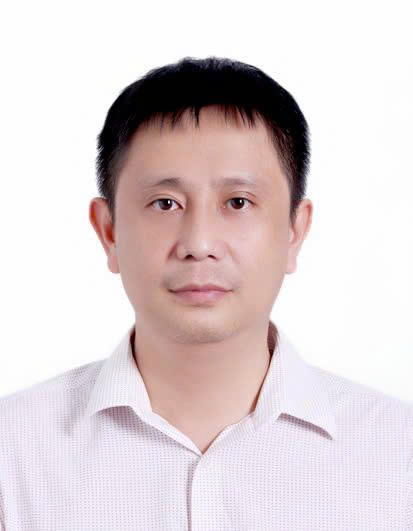
\includegraphics[width=1in,height=1.25in,clip,keepaspectratio]{authors/pham.jpg}}]{Minh Tuan Pham}
received the Ph.D. degree in Computational Science and Engineering from Nagoya
University, Japan, in 2012. He is currently a faculty member and researcher with
the Faculty of Information Technology, The University of Danang - University of
Science and Technology, Danang, Vietnam, where he serves as the Head of the
Artificial Intelligence and Advanced Computing Research Group. He is also the
Director of the International Collegiate Programming Contest (ICPC) Central
Vietnam Region. His research interests include Artificial Intelligence, Soft
Computation, and Geometric Algebra.
\end{IEEEbiography}

\begin{IEEEbiography}[{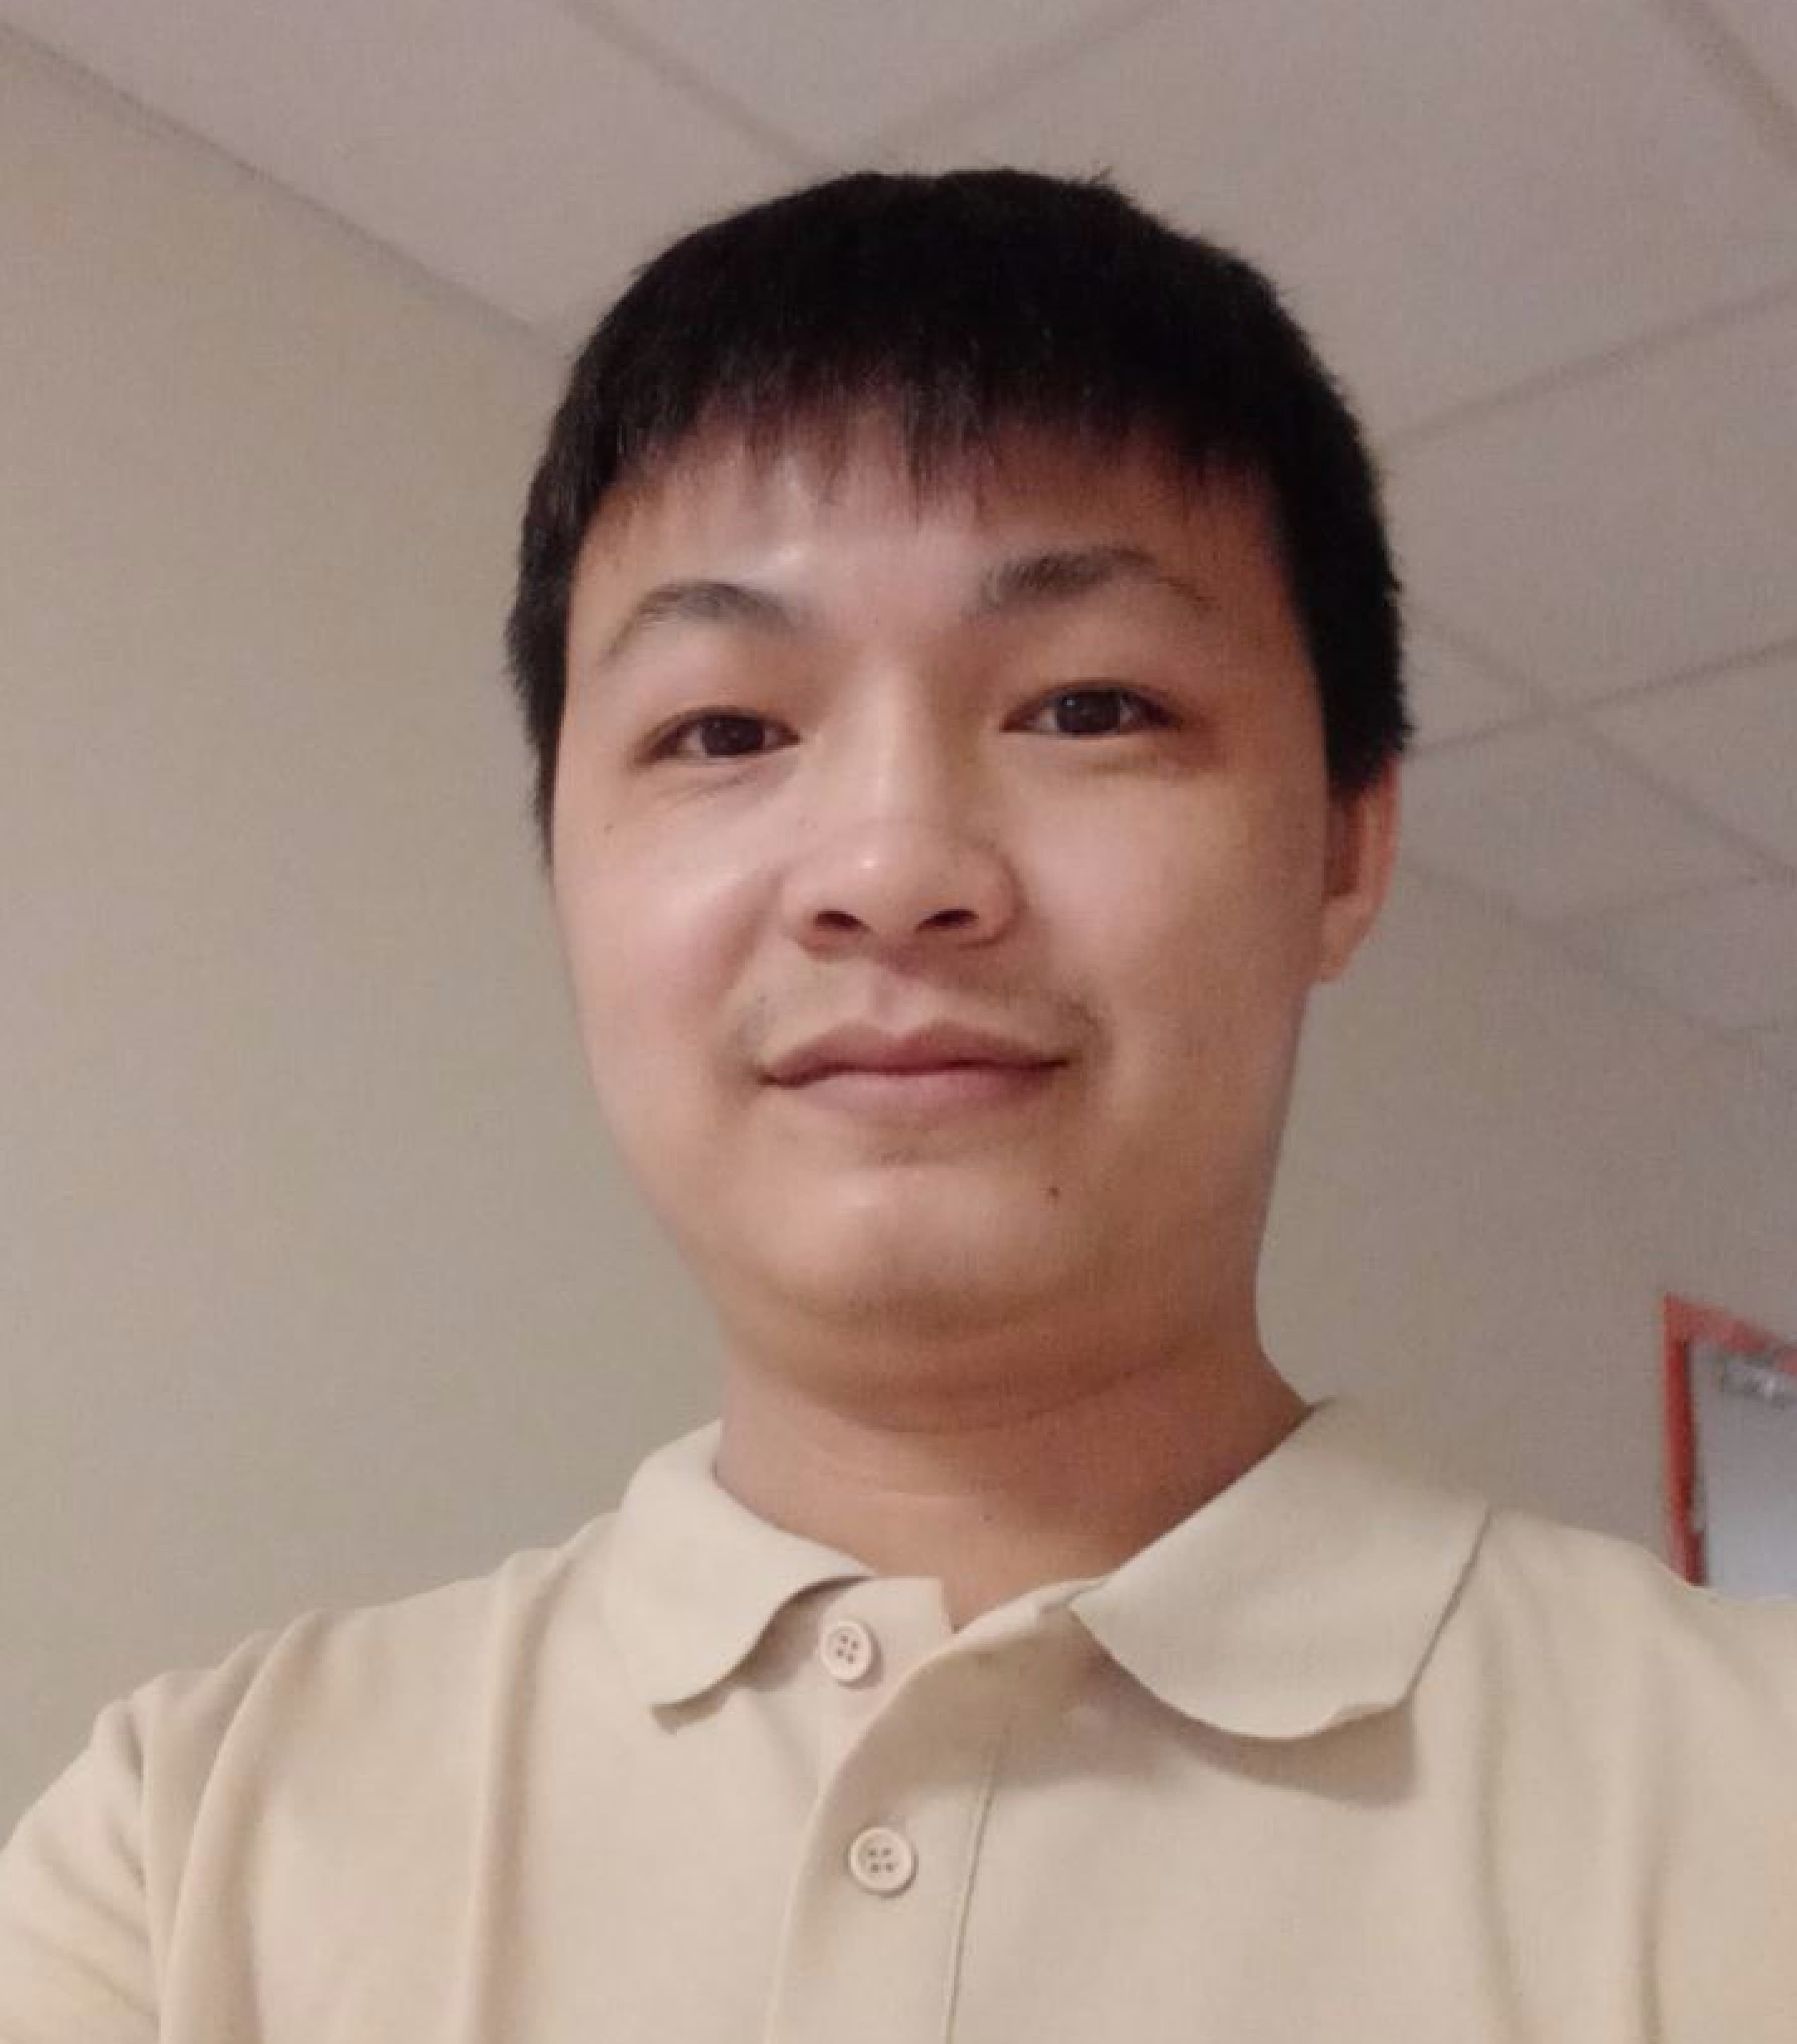
\includegraphics[width=1in,height=1.25in,clip,keepaspectratio]{authors/do.jpg}}]{Phuc Hao Do}
received the Ph.D. degree in Telecommunications and Networks from The
Bonch-Bruevich Saint Petersburg State University of Telecommunications, Saint
Petersburg, Russia, in 2026, and the M.S. degree in Computer Science from The
University of Danang - University of Science and Technology, Danang, Vietnam, in
2017. He is currently affiliated with both institutions. His doctoral research
focused on applying advanced AI and quantum computing principles to
next-generation satellite communication systems. His current research interests
include Federated Learning for secure, distributed intelligence in satellite
constellations, Quantum Machine Learning for network routing and resource
allocation, and AI-driven traffic management. He has published in reputable IEEE
journals and international conferences.
\end{IEEEbiography}

\begin{IEEEbiography}[{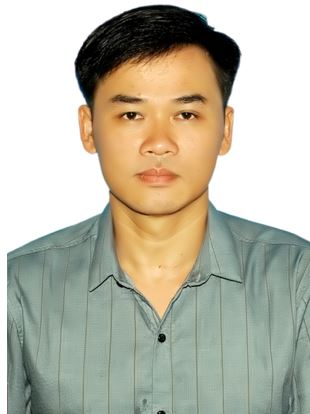
\includegraphics[width=1in,height=1.25in,clip,keepaspectratio]{authors/van.jpg}}]{Nguyen Nang Hung Van}
received the Ph.D. degree in Computer Science from The University of Danang,
Vietnam, in 2021. He is currently a lecturer with The University of Danang -
University of Science and Technology, Danang, Vietnam. His research interests
include Artificial Intelligence, Machine Learning, Geometric Algebra, and
Computer Networking.
\end{IEEEbiography}

\begin{IEEEbiography}[{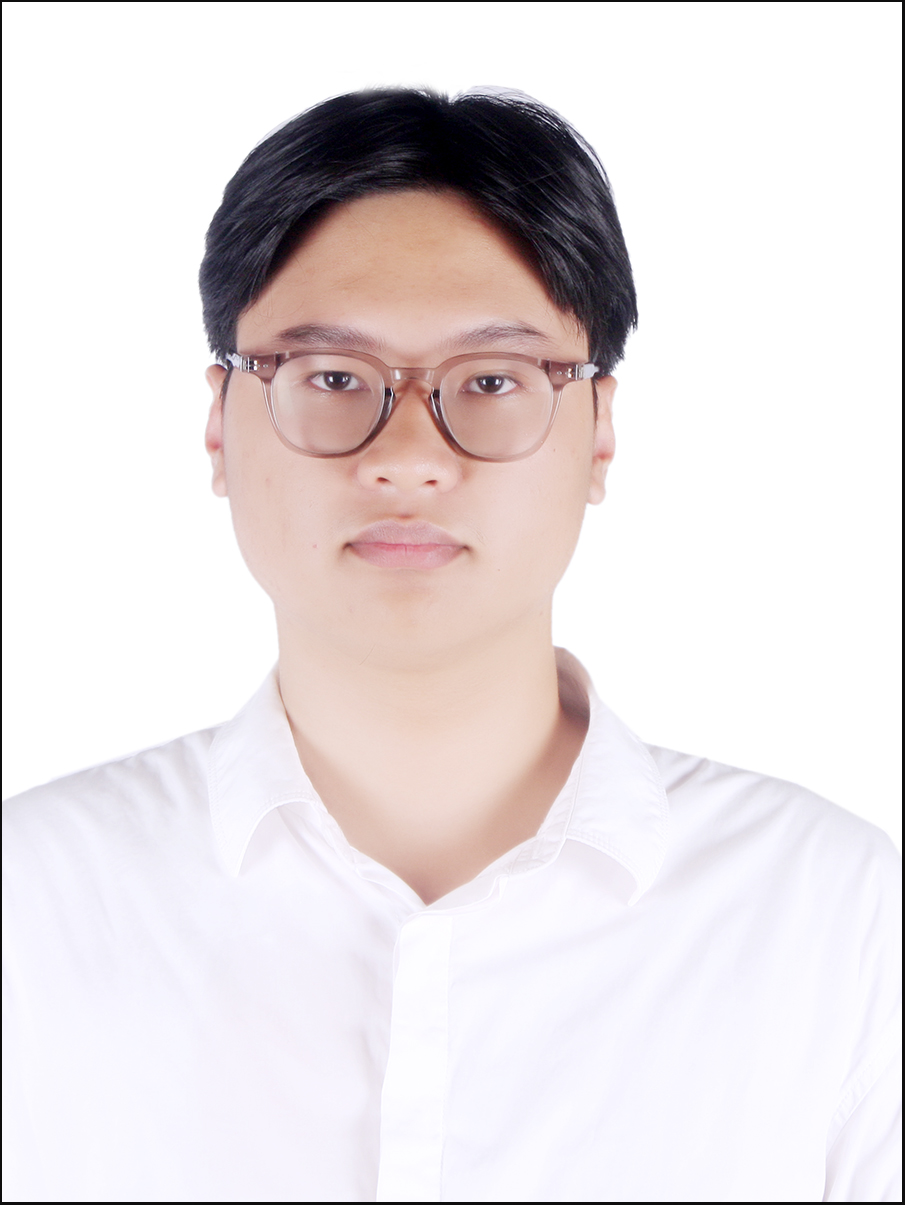
\includegraphics[width=1in,height=1.25in,clip,keepaspectratio]{authors/nguyen.jpg}}]{Quang Anh Nguyen}
is currently pursuing the B.S. degree in Information Technology with The
University of Danang - University of Science and Technology, Danang, Vietnam,
where he is a third-year undergraduate student. His research interests include
satellite technologies, Artificial Intelligence and Machine Learning
applications, and embedded systems.
\end{IEEEbiography}

\begin{IEEEbiography}[{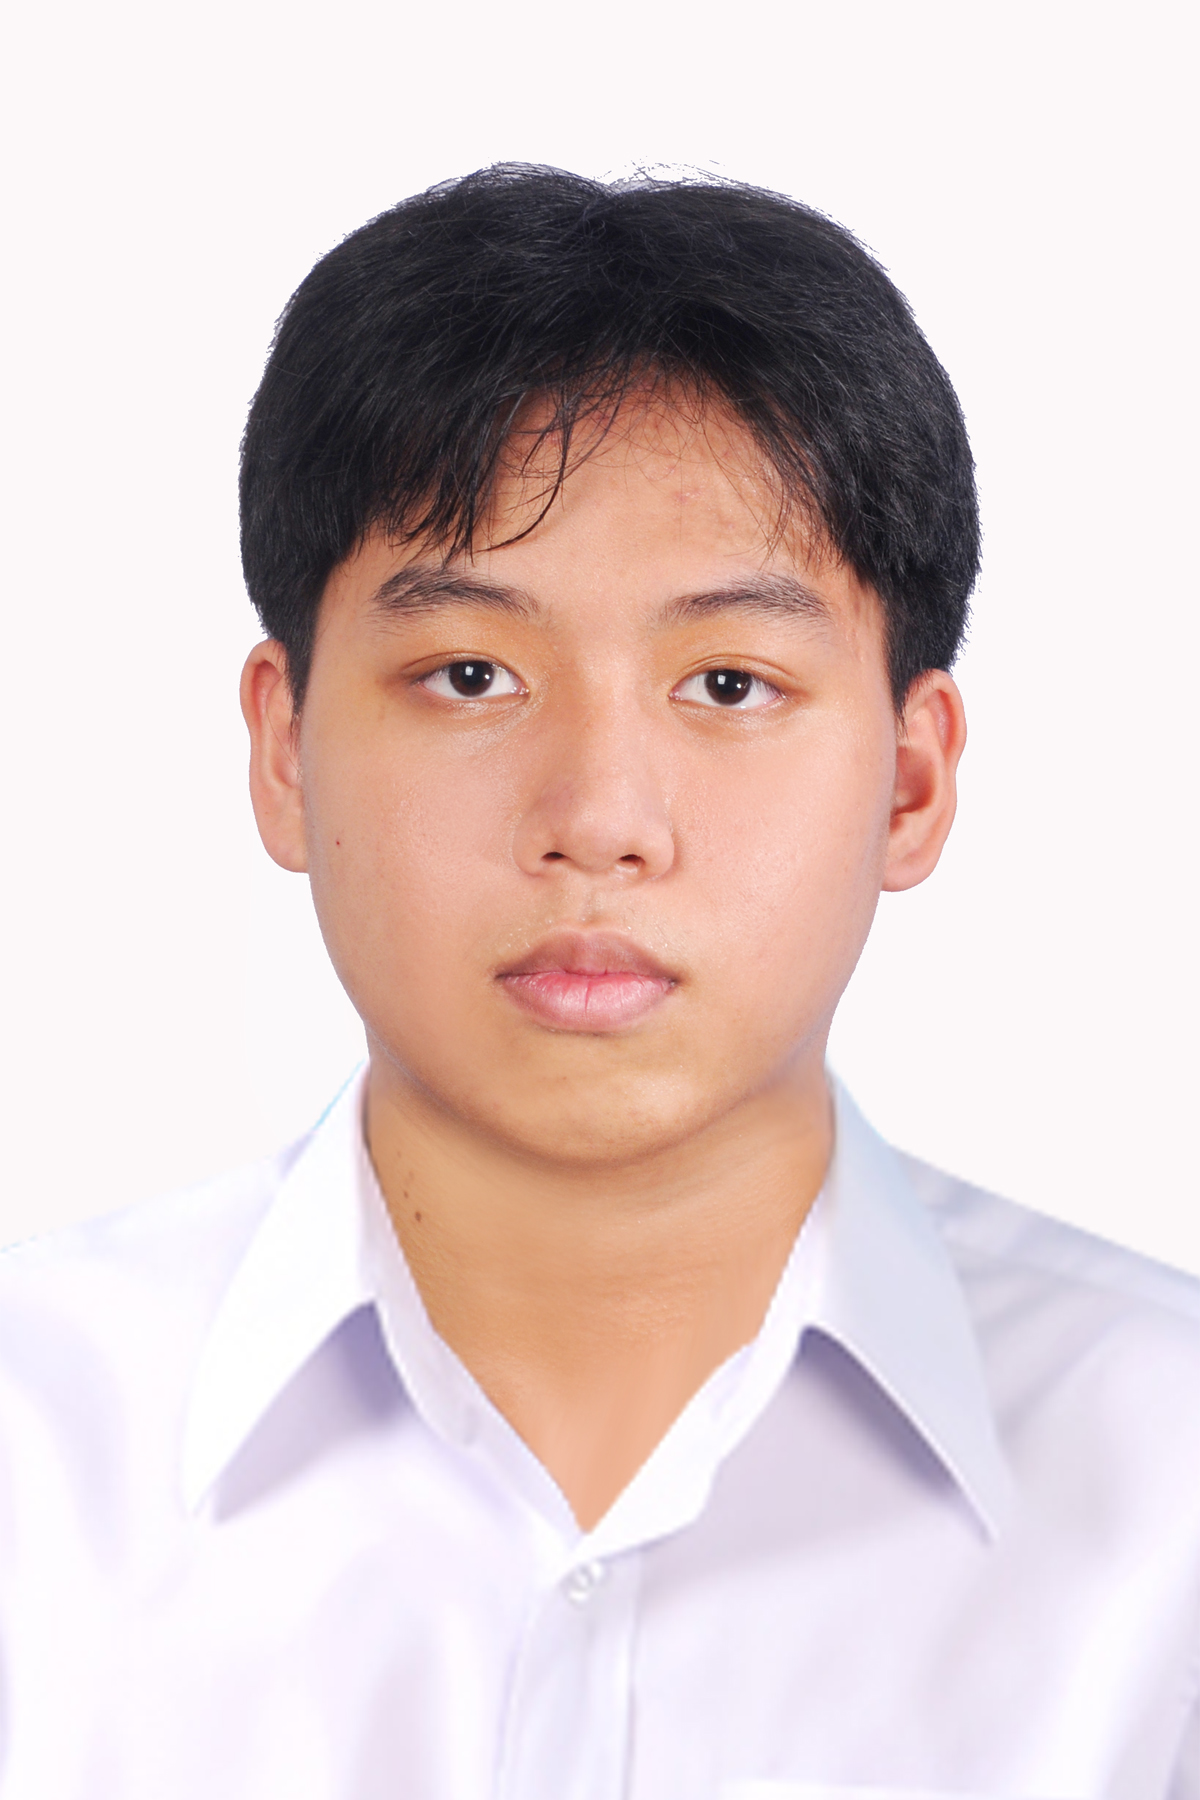
\includegraphics[width=1in,height=1.25in,clip,keepaspectratio]{authors/vo.jpg}}]{Quan Tran Anh Vo}
is currently pursuing an undergraduate degree at The University of Danang -
University of Science and Technology, Danang, Vietnam. He serves as a lead
researcher in university scientific research programs. His research interests
include Artificial Intelligence, Quantum Machine Learning, and Network Security.
\end{IEEEbiography}
